\documentclass{beamer}

\mode<presentation>
{
  \usetheme{Frankfurt}
  \usecolortheme{orchid}
  \setbeamercovered{invisible}
  \setbeamertemplate{footline}[frame number]
}

\usepackage[english]{babel}
\usepackage[latin1]{inputenc}
\usepackage{times}
\usepackage[T1]{fontenc}
\usepackage{tikz}
\usepackage{array}
\usepackage{cancel}


\usetikzlibrary{shapes,backgrounds}

\def\multiset#1#2{\ensuremath{\left(\kern-.3em\left(\genfrac{}{}{0pt}{}{#1}{#2}\right)\kern-.3em\right)}}

\def\blue{\color{blue}~}
\def\black{\color{black}~}
\def\bl[#1]#2{\begin{block}{#1}#2\end{block}}
\def\integers{\mathbb{Z}}
\def\enumb{\begin{enumerate}}
\def\enume{\end{enumerate}}
\def\itemb{\begin{itemize}}
\def\iteme{\end{itemize}}


\usepackage{remreset}
\makeatletter
\@removefromreset{subsection}{section}
\makeatother
\setcounter{subsection}{1}

\title{Discrete Mathematics, Section 001, Fall 2016}
\subtitle{Lecture 10: Contrapositive, Contradiction, Smallest counterexample}
\date{October 17, 2016}

\author[Zsolt]{Zsolt Pajor-Gyulai \\ \texttt{zsolt@cims.nyu.edu}}

\pgfdeclareimage[height=1cm]{NYUlogo}{NYUlogo.jpg}

\institute[NYU] 
{
\normalsize Courant Institute of Mathematical Sciences
}
\titlegraphic{\pgfuseimage{NYUlogo}}

\begin{document}

\begin{frame}
  \titlepage
\end{frame}

\AtBeginSection[]
{
\begin{frame}
\frametitle{Outline}
\tableofcontents[currentsection]
\end{frame}}

\section{Contrapositive and contradiction}

\begin{frame}{Proof by contrapositive}
So far we learned to prove $A\Rightarrow B$ statements directly. Here is an alternative way:
\[
a\rightarrow b=\neg a\vee b=\neg a\vee \neg(\neg b)=\neg(\neg b)\vee\neg a=\neg b\to \neg a
\]
where $=$ now means logical equivalence. Therefore,
\bl[]{
\[
A\Rightarrow B\qquad\textrm{is the same as}\qquad (\textrm{not }B)\Rightarrow (\textrm{not }A)
\]
}
\bl[Proof by contrapositive]{
To prove `If $A$, then $B$': Assume $(\neg B)$ and work to prove $(\neg A)$.
}
\end{frame}

\begin{frame}{Proof by contrapositive}
\bl[Proposition]{
Let $R$ be an equivalence relation on a set $A$ and let $a,b\in A$. If $a\cancel{R} b$, then $[a]\cap[b]=\emptyset$.
}

\begin{proof}
Let $R$ be an equivalece relation on a set $A$ and let $a,b\in A$. We prove the contrapositive of the statement.

~~~~ Suppose $[a]\cap[b]\neq\emptyset$. \only<2>{\color{blue}}\uncover<2->{Thus there is an $x\in[a]\cap[b]$; that is, $x\in [a]$ and $x\in [b]$.}\only<2>{\color{black}}\only<3>{\color{blue}}\uncover<3->{ Hence $x R a$ and $x R b$. By symmety $a R x$, and since $x R b$, by transitivity}\color{black}~we have $a R b$.
\end{proof}

\uncover<4>{To see the advantage, try thinking of a direct proof!

\center{Formulate some theorems like this in Problem 1 and prove one in Problem 2 on the Worksheet!}}
\end{frame}

\begin{frame}{Reductio ad absurdum (Proof by contradiction)}
Note that
\begin{align*}
a\rightarrow b&=\neg a \vee b=\neg a\vee b\vee False=\\
&=\neg(a\wedge\neg b)\vee False=(a\wedge\neg b)\rightarrow False
\end{align*}
where $=$ again means logical equivalence.
\bl[]{\vspace{-0.5cm}
\[
A\Rightarrow B\qquad\textrm{is the same as}\qquad(A\textrm{ and } not(B))\Rightarrow Impossible
\]}

  What on earth does this mean?
  \itemb
  \item If $A$ and $not(B)$ are simultaneously true that implies the impossible.
  \item In other words $A\Rightarrow B$ is the same as $A$ and $not(B)$ being impossible to be simultaneously true.
  \iteme
\end{frame}

\begin{frame}{Reductio ad absurdum (Proof by contradiction)}
\bl[]{\vspace{-0.5cm}
\[
A\Rightarrow B\qquad\textrm{is the same as}\qquad(A\textrm{ and } (\textrm{not }B))\Rightarrow Impossible
\]}
 If $A$ and (not $B$) are both true that implies the impossible.

  
\bl[Proof by contradiction]{
 To prove ``If $A$ then $B$'': \\
 \itemb
 \item We assume the conditions in $A$.\\
 \item Suppose for the sake of contradiction, (not $B$).\\
\item  Argue until we reach a contradiction (something impossible).\\ 
 \iteme
 ~~~~Thus we have reached a contradiction. Therefore the \\
 ~~~~~supposition (not $B$) must be false. Hence $B$ is true.
}
The last two sentece is often abbreviated by $\Rightarrow\Leftarrow$.
\end{frame}

\begin{frame}{Reductio ad absurdum (Proof by contradiction)}
\bl[]{\vspace{-0.5cm}
\[
A\Rightarrow B\qquad\textrm{is the same as}\qquad(A\textrm{ and } (\textrm{not }B))\Rightarrow Impossible
\]}

If $A$ and (not $B$) are both true that implies the impossible.

\bl[Proof by contradiction]{
 To prove ``If $A$ then $B$'': \\
 \itemb
\item We assume the conditions in $A$.
\item Suppose for the sake of contradiction, (not $B$).
\item Argue until we reach a contradiction (something impossible).
\iteme
~~~~ $\Rightarrow\Leftarrow$.
}
\end{frame}

\begin{frame}{Reductio ad absurdum (Proof by contradiction)}
\bl[Proposition]{
No integer is both even and odd
}
\begin{proof}
Let $x$ be an integer.

~~~~ Suppose, for the sake of contradiction, that $x$ is both even and odd.

\only<2>{\color{blue}}\uncover<2->{~~~~ Since $x$ is even, we know $2|x$; that is, there is an integer $a$ such that $x=2a$. Since $x$ is odd, we know that there is an integer $b$ such that $x=2b+1$.}

\only<3>{\color{blue}}\uncover<3->{~~~~ Therefore $2a=2b+1$. Dividing both sides by $2$ gives $a-b=\frac{1}{2}$. Note that $a-b$ is an integer since $a$ and $b$ are integers. However, $\frac{1}{2}$ is not an integer.}\color{black} $\Rightarrow\Leftarrow$

Therefore $x$ is not both even and odd, and the propostition is proved.
\end{proof}

\end{frame}

\begin{frame}
\center Now practice how to set up such proofs by doing Problem 3 on the worksheet!
\end{frame}

\begin{frame}{Proving that a set is empty}
\bl[Proposition]{
\only<1>{No integer is both even and odd}
\only<2->{Let \vspace{-0.4cm}
\[
X=\{x\in\mathbb{Z}: \textrm{$x$ is even}\},\qquad Y=\{x\in\mathbb{Z}: \textrm{$x$ is odd}\}.\vspace{-0.3cm}
\]\\
Then $X\cap Y=\emptyset$.
}}
\uncover<3->{
\bl[Proving that a set is empty]{
To prove a set is empty:\\
~~~~Assume the set is nonempty and argue to a contradiction.
}}
\end{frame}

\begin{frame}{Proving uniqueness}
\bl[Proving uniqueness]{
To prove there is at most one object that satisfies certain conditions:\\
~~~~Suppose there are two different objects, $x$ and $y$, that satisfy the conditions and argue to a contradiction.
}

\bl[Proposition]{Let $a$ and $b$ be numbers with $a\neq 0$. There is at most one number $x$ with $ax+b=0$.}

\end{frame}

\begin{frame}{Proving uniqueness}
\bl[Proposition]{Let $a$ and $b$ be numbers with $a\neq 0$. There is at most one number $x$ with $ax+b=0$.}

\begin{proof}
Suppose there are two different numbers $x$ and $y$ such that $ax+b=0$ and $ay+b=0$. This gives
\[
ax+b=ay+b.
\]
Substracting $b$ from both sides gives $ax=ay$. Since $a\neq 0$, we can divide both sides by $a$ to give $x=y$. $\Rightarrow\Leftarrow$.
\end{proof}
\center Now practice writing some proofs like this by doing Problem 4 on the worksheet!
\end{frame}

\begin{frame}{Caveats}
\itemb
\item Proof by contradiction is often easier than the direct proof because there are more things to work with.
\item Sometimes this is not required though.
\item Here is how to tell when you can simplify a proof of ``If $A$ then $B$'' by contradiction.

\itemb
\item You assumed $A$ and (not $B$), but you only used $A$ and reached $B$ and (not $B$). Then you really have a direct proof and you should remove the extraneous proof by contradiction apparatus.
\item You assumed $A$ and (not $B$), but you only used (not $B$), and the contradiction you reached was $A$ and (not $A$). Then you really have a proof by contrapositive and you should rewrite the proof in that form.
\iteme
\iteme
\end{frame}

\begin{frame}[t]{Sudoku}
\vspace{-0.2cm}
With Sudoku puzzles, countradiction reasoning is what you do.
\begin{figure}
\begin{tikzpicture}[scale=0.8]
\foreach \x in {0,1,2,3,4,5,6,7,8,9}
	{
		\draw (\x,0) -- (\x, 3);
	}
	
\foreach \x in {0,1,2,3}
	{
		\draw (0,\x) -- (9,\x);
	}
	
\foreach \x in {0, 3}
	{
		\draw[line width=3pt] (0,\x)--(9,\x);
	}
	
\foreach \x in {0,3,6,9}
	{
		\draw[line width=3pt] (\x,0) -- (\x, 3);
	}
	
\node at (0.5,0.5) {$5$};
\node at (1.5,0.5) {$6$};
\node at (2.5,0.5) {$7$};
\node at (4.5,0.5) {$2$};
\node at (5.5,0.5) {$8$};

\node at (5.5,1.5) {$3$};
\node at (7.5,1.5) {$1$};

\node at (3.5,2.5) {$4$};
\node at (5.5,2.5) {$9$};
\node at (8.5,2.5) {$8$};

\only<2>{\node at (3.5,0.5) {$\color{blue}1\color{black}$};}
\only<3>{\node at (4.5,2.5) {$\color{red}1\color{black}$};}
\only<4>{\node at (4.5,1.5) {$\color{red}1\color{black}$};}
\only<5>{\node at (3.5,1.5) {$\color{red}1\color{black}$};}
\end{tikzpicture}
\end{figure}
\uncover<2->{\bl[Claim]{The $1$ for the middle box must go to the left on the $2$ in the bottom row.}}
\uncover<2->{\begin{proof}
\only<3>{Suppose $1$ goes in the top row. Then the $1$ for the left box cannot be in the top row and cannot be in the middle row and cannot be in the bottom row. $\Rightarrow\Leftarrow$.}
\only<4->{Suppose $1$ goes in the middle row. But then we would have two $1$s in the middle row. $\Rightarrow\Leftarrow$.}
\end{proof}}

\end{frame}

\section{Smallest Counterexample}

\begin{frame}{Motivation}
\itemb
\item Proving something by contradiction is essentially assuming there is a counterexample and showing that it would break the universe.
\item You can view this really as a proof by the lack of counterexample.

\item Sometimes there is a natural ordering associated with certain statements. For example, when we prove something for all natural numbers, then these natural numbers are ordered by the usual ordering. 
\item In these cases if there is a counterexample, e.g. a natural number for which the statement is not true, then there has to be a smallest such counterexample.
\item This gives us an extra tool to work with as we can use that for anything smaller than the smaller counterexample, the result holds.
\iteme
\end{frame}

\begin{frame}{Example}
\bl[Proposition]{Every natural number is either even or odd}

\begin{proof}
Suppose, for the sake of contradiction, that there were an integer $x$ that is neither even nor odd. \color{blue}\uncover<2->{ So there is no integer $b$ with $x=2b$, and there is no integer $b$ such that $x=2b+1$.}\color{black} $\dots$ $\Rightarrow\Leftarrow$. Therefore every natural is either even or odd.
\end{proof}
\uncover<3->{\center We are stuck here, we have to come up with something more!}
\end{frame}

\begin{frame}
\bl[Proposition]{Every natural number is either even or odd}

\begin{proof}
Suppose, for the sake of contradiction, that there were an natural $x$ that is neither even nor odd. \only<2>{\color{blue}}\uncover<2->{Then there is a SMALLEST natural number, $x$, that is neither even nor odd.}

\only<4>{\color{blue}}\uncover<4->{~~~~We know $x\neq 0$, because $0$ is even. Therefore $x\geq 1$.}

~~~~\color{black}\only<3>{\color{blue}}\uncover<3->{Since \only<5>{\color{blue}}\uncover<5->{$0\leq$}\uncover<5->{\color{black}} $x-1$ is a smaller natural than $x$,  we know that $x-1$ is either even or odd.}
\uncover<6->{\itemb
\uncover<6->{\only<6>{\color{blue}}\item Suppose $x-1$ is odd, then $x-1=2a+1$ for some $a\in\mathbb{Z}$. Thus $x=2a+2=2(a+1)$ and so $x$ is even.$\Rightarrow\Leftarrow$.}
\uncover<7->{\item \only<7>{\color{blue}} Suppose $x-1$ is even, then $x-1=2a$ for some $a\in\mathbb{Z}$. Thus $x=2a+1$ and so $x$ is odd.$\Rightarrow\Leftarrow$.}
\iteme}
\only<8>{\color{blue}}\uncover<8>{In every case, }\color{black} we have a contradiction, so the supposition is false and the proposition is proved.
\end{proof}
\end{frame}

\begin{frame}{Extension to all integers}
\bl[Corollary]{Every integer is either even or odd.}
\begin{proof}
Let $x\in\mathbb{Z}$. If $x\geq 0$ then the previous proposition applies and $x$ is either even or odd. Otherwise $x<0$ in which case $-x>0$ and so $-x$ is either even or odd.
\itemb
\item If $-x$ is even, then $-x=2a$ for some $a\in\mathbb{Z}$. But then $x=-2a=2(-a)$ and $x$ is even as $-a\in\mathbb{Z}$.
\item If $-x$ is odd then $-x=2a+1$ for some $a\in\mathbb{Z}$. But then $x=-2a-1=2(-a-1)+1$ and $x$ is odd as $-a-1\in\mathbb{Z}$.
\iteme
In every case, $x$ is either even or odd.
\end{proof}
\end{frame}

\begin{frame}{Proof template for smallest counterexample}
\bl[Proof by smallest counterexample]{
\enumb
\item First, let $x$ be a smallest counterexample to the result we are trying to prove. It must be clear that there can be such an $x$.
\item Second, rule out $x$ being the very smallest possibility. This is usually easy and is called the basis step.
\item Third consider an instant $x'$ of the result that is just smaller than $x$. Use the fact that according to the assumption, the result is true for $x'$ but false for $x$, to reach $\Rightarrow\Leftarrow$.
\enume
}
\center Try to write a proof like this yourself by doing Problem 5  on the worksheet!
\end{frame}

\begin{frame}{Another example}
\bl[Proposition]{
Let $n$ be a positive integer. Then $\sum_{k=1}^n(2k-1)=n^2$.
}
\bl[Proof]{
Suppose the claim is false. Then there is a smallest positive integer $x$ for which\vspace{-0.7cm}
\[
\sum_{k=1}^x(2k-1)\neq x^2.
\]\vspace{-0.5cm}
\\
Clearly $x\neq 1$, because $1=1^2$ and therefore $x>1$. Since $x$ was the smallest counterexample,\vspace{-0.4cm}
\[
\sum_{k=1}^{x-1}(2k-1)= (x-1)^2.
\]
[...]
}
\end{frame}

\begin{frame}{Another example}
\bl[Proposition]{
Let $n$ be a positive integer. Then $\sum_{k=1}^n(2k-1)=n^2$.
}
\begin{proof}

[...]
\[
\sum_{k=1}^{x-1}(2k-1)= (x-1)^2.
\]
Add $2x-1$ to both sides to get\vspace{-0.3cm}
\begin{align*}
\sum_{k=1}^{x}(2k-1)&= (x-1)^2+(2x-1)=\\
&=x^2-2x+1+2x-1=x^2.
\end{align*}\vspace{-0.5cm}

contradicting that $x$ is a counterexample. $\Rightarrow\Leftarrow$.
\end{proof}
\end{frame}

\begin{frame}{The well ordering principle}
The following statement is crucial in the above proofs.
\bl[Well ordering principle]{Every nonempty set of natural numbers contains a least element.}
For example,
\itemb
\item $P=\{x\in\mathbb{N}: x\textrm{ is prime}\}$. Least element is $2$.
\item $X=\{x\in\mathbb{N}: x\textrm{ is neither even nor odd}\}$. This is of course the emptyset, but if it was not, there would be a smallest element.
\iteme
However,
\itemb
\item $Y=\{y\in\mathbb{Q}: y\geq 0, y\notin\mathbb{Z}\}$. This has no smallest element, if there was, you could prove that every rational is an integer, which is obviously false.
\iteme
The WOP is a property of the natural numbers but not a property of the integers or the rationals.
\end{frame}

\begin{frame}{The well ordering principle}
\bl[To prove a statement about the natural numbers]{
\enumb
\item Suppose for the sake of contradiction, that the statement is false, let $X\subseteq \mathbb{N}$ to be the set of counterexamples.
\item By assumption $X\neq\emptyset$ and thus by the well ordering principle it has a smallest element.
\item We know $x\neq 0$ because (show result holds for $0$).
\item Therefore $x-1\in\mathbb{N}$ and the statement is true for $x-1$. 
\item (Argue for contradiction) $\Rightarrow\Leftarrow$.
\enume
}
\center In the remaining time, practice this by doing Problems 6-8 on the worksheet.
\end{frame}
\end{document}